\chapter{Phân tích và thiết kế}
\label{ch:thietke}

\section{Phân tích bài toán và yêu cầu}

\subsection{Đầu vào và đầu ra của hệ thống}

\textbf{Đầu vào} của hệ thống gợi ý trung tâm bao gồm hồ sơ năng lực do học sinh nhập:
\begin{itemize}[leftmargin=1.6em, itemsep=2pt]
  \item Điểm thi từng môn học (thang 10) và điểm học bạ trung bình các môn.
  \item Tổ hợp môn xét tuyển mà học sinh có thể sử dụng (ví dụ: A00 --- Toán, Lý, Hóa).
  \item Nhóm ngành đào tạo ưu tiên và khu vực địa lý mong muốn trong số 15 nhóm ngành và 3 vùng miền.
\end{itemize}

\textbf{Đầu ra} là danh sách tối đa 30 nguyện vọng (mỗi nguyện vọng là một bộ: trường, ngành, tổ hợp, phương thức) được sắp xếp theo xác suất trúng tuyển giảm dần và phân thành 3 tầng trực quan: Tầng \textbf{An toàn} ($p \ge 0{,}80$) dùng làm phương án dự phòng chắc chắn; tầng \textbf{Vừa sức} ($0{,}40 \le p < 0{,}80$) là nhóm lựa chọn chính phù hợp năng lực; tầng \textbf{Thử sức} ($p < 0{,}40$) là nhóm kỳ vọng cao dành cho ngành yêu thích.

\subsection{Yêu cầu chức năng}

Hệ thống bao gồm 11 ca sử dụng \en{(Use Case)} chính, chia theo ba nhóm tác nhân: Khách (tra cứu, xem chi tiết trường), Học sinh đã đăng nhập (nhập hồ sơ điểm, nhận gợi ý AI, xem lời giải thích, so sánh và lưu nguyện vọng) và Quản trị viên (cập nhật dữ liệu năm mới, huấn luyện lại mô hình, xem thống kê). Hai ca sử dụng trung tâm có AI tham gia là UC-05 (Nhận gợi ý trường, ngành) và UC-10 (Huấn luyện lại mô hình). Toàn cảnh quan hệ giữa các tác nhân và các ca sử dụng được thể hiện ở Hình~\ref{fig:usecase}.

\begin{figure}[H]
\centering
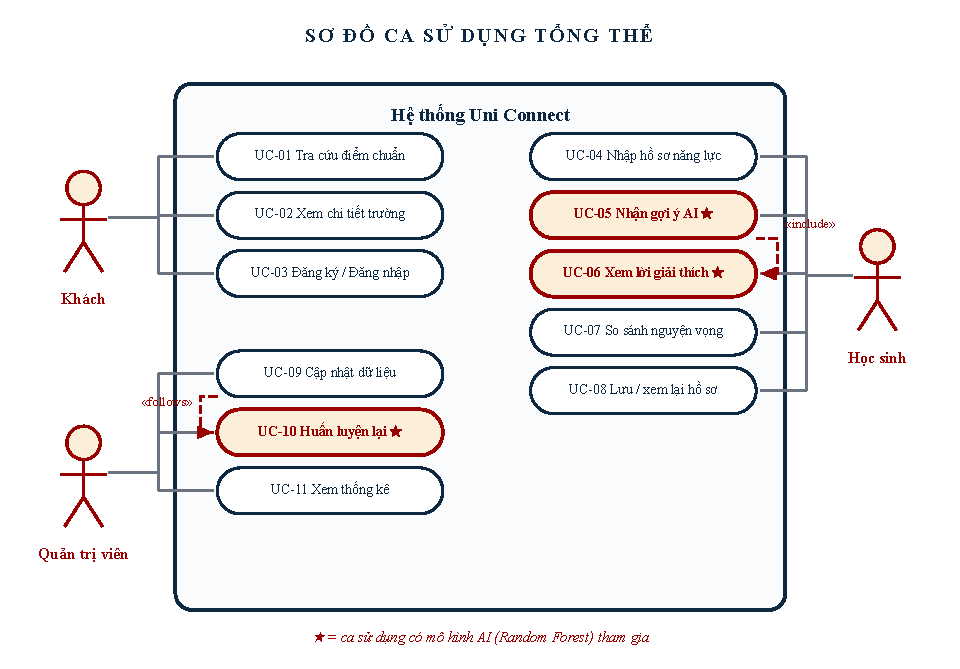
\includegraphics[width=\textwidth]{figs/svg/h-usecase.pdf}
\caption{Sơ đồ ca sử dụng (Use Case) tổng thể của hệ thống Uni Connect.}
\label{fig:usecase}
\end{figure}

Mười một ca sử dụng trên được phân rã thành năm nhóm chức năng theo mô hình cây như Hình~\ref{fig:bfd}. Cách phân rã này bám sát cấu trúc thư mục mã nguồn thật của đồ án: mỗi nhóm chức năng tương ứng một ứng dụng Django độc lập.

\begin{figure}[H]
\centering
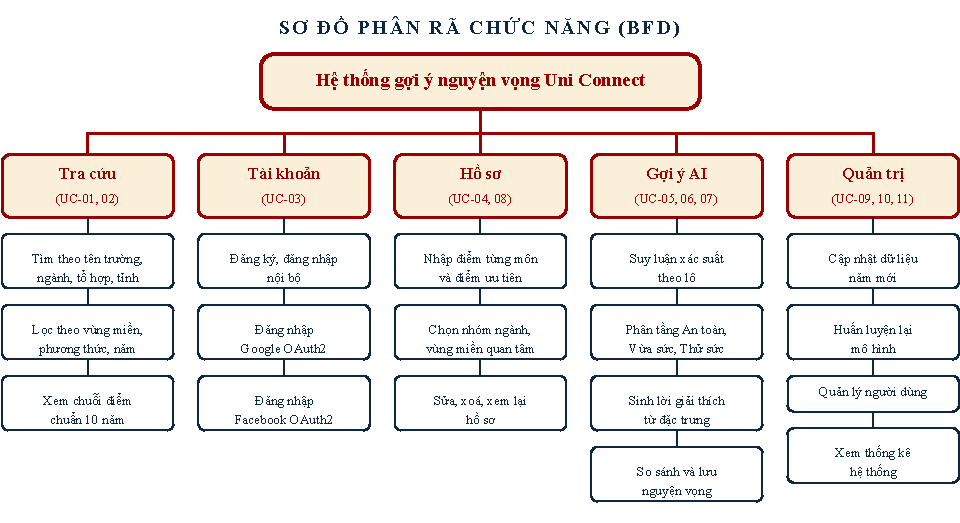
\includegraphics[width=\textwidth]{figs/svg/h-bfd.pdf}
\caption{Sơ đồ phân rã chức năng (BFD) của hệ thống Uni Connect.}
\label{fig:bfd}
\end{figure}

\textbf{Tiêu chí hệ thống chạy đúng:}
\begin{itemize}[leftmargin=1.6em, itemsep=2pt]
  \item Mọi điểm chuẩn hiển thị trên giao diện phải trùng khớp tuyệt đối với bản ghi đã lưu trong cơ sở dữ liệu.
  \item Với cùng một hồ sơ đầu vào, danh sách gợi ý sinh ra phải nhất quán và có thứ tự xếp hạng ổn định.
  \item Ngưỡng phân tầng 0,80 và 0,40 được khai báo công khai rõ ràng trên giao diện, không để người dùng tự ước đoán.
\end{itemize}

\subsection{Yêu cầu phi chức năng}
\label{sec:nfr}

\begin{itemize}[leftmargin=1.6em, itemsep=2pt]
  \item \textbf{Hiệu năng} (PC-01): Trang gợi ý AI phải phản hồi trong vòng dưới 3 giây trên hạ tầng máy chủ thông thường; mô hình \code{model.pkl} (~52~MB) chỉ nạp một lần vào RAM khi khởi động tiến trình, không đọc lại đĩa cứng mỗi lượt truy vấn.
  \item \textbf{Độ tin cậy:} Mọi lỗi liên quan đến mô hình (thiếu file, sai lệch phiên bản thư viện) đều không được gây lỗi hệ thống 500. Hệ thống tự động chuyển sang chế độ dự phòng (xếp hạng bằng \code{margin} thuần) và ghi rõ trạng thái ``chưa dùng mô hình AI''.
  \item \textbf{Khả năng mở rộng:} Cơ chế cửa sổ trượt cho phép cập nhật dữ liệu năm mới (ví dụ: năm 2026) mà không cần thay đổi cấu trúc bảng hay viết lại mã nguồn xử lý.
\end{itemize}

\section{Thiết kế kiến trúc hệ thống}

Kiến trúc tổng thể của hệ thống Uni Connect được trình bày ở Hình~\ref{fig:kientruc}. Dữ liệu vận hành theo luồng khép kín gồm 4 tầng chính.

\begin{figure}[H]
\centering
\resizebox{\textwidth}{!}{%
\begin{tikzpicture}[node distance=10mm and 12mm]
  \node[objbox] (crawl) {Thu thập\\(crawler, CSV)};
  \node[clsbox, right=of crawl] (db) {CSDL MySQL\\(15 bảng quan hệ)};
  \node[clsbox, right=of db] (model) {Mô hình AI\\(Random Forest)};
  \node[clsbox, right=of model] (web) {Django Web\\(tra cứu, gợi ý)};
  \node[objbox, right=of web] (user) {Học sinh,\\quản trị viên};
  \draw[flowarr] (crawl) -- (db);
  \draw[flowarr] (db) -- (model);
  \draw[flowarr] (model) -- (web);
  \draw[flowarr] (web) -- (user);
  \draw[flowarr] (user) |- ($(web.south)+(0,-6mm)$) -| (web);
\end{tikzpicture}}
\caption{Sơ đồ kiến trúc tổng thể của hệ thống gợi ý nguyện vọng Uni Connect.}
\label{fig:kientruc}
\end{figure}

Luồng hoạt động cụ thể như sau: (1) Bộ thu thập ngoại tuyến \code{crawl_diemchuan.py} tự động tải, làm sạch dữ liệu và xuất ra các file CSV chuẩn; (2) Script \code{import_mysql.py} nạp dữ liệu vào CSDL MySQL; (3) Pipeline huấn luyện \code{gen_dataset.py} trích xuất đặc trưng và \code{train.py} sinh ra mô hình \code{model.pkl}; (4) Ứng dụng web Django phục vụ người dùng cuối, gọi mô hình khi có yêu cầu gợi ý thông qua module suy luận \code{predict.py}.

\section{Sơ đồ luồng xử lý nghiệp vụ}

\subsection{UC-03 Đăng ký / Đăng nhập}

Luồng xử lý tài khoản bao gồm khóa tạm theo tỷ lệ sai khi đăng nhập, cơ chế dự phòng cho dịch vụ.

\begin{figure}[H]
\centering
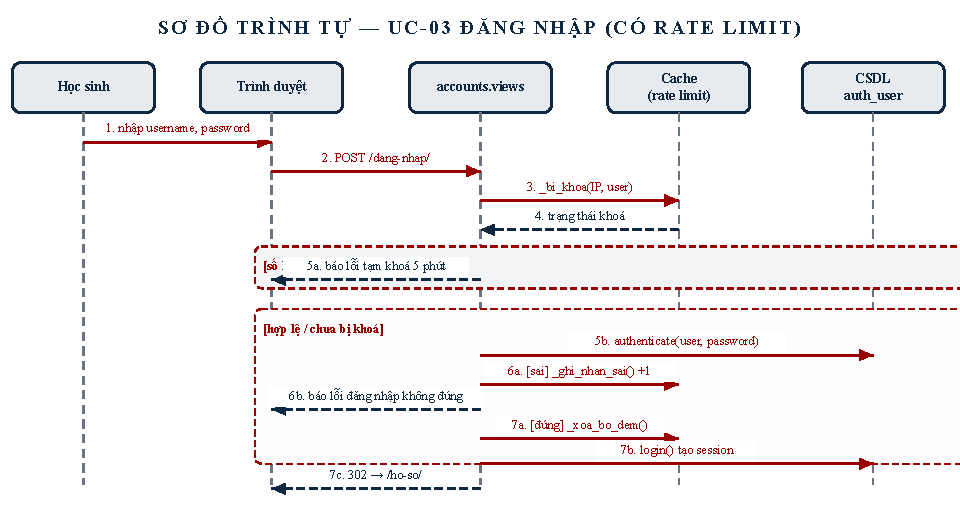
\includegraphics[width=\textwidth]{figs/svg/h-seq-dangnhap.pdf}
\caption{Sơ đồ trình tự UC-03 Đăng nhập (với cơ chế rate limit và câu trả lời dự phòng).}
\label{fig:seq-dangnhap}
\end{figure}

\subsection{UC-05 Nhận gợi ý (AI)}

Luồng xử lý nhận gợi ý dung sự khía cạnh: mô hình AI khi sẵn sàng, cơ chế dự phòng xếp hạng theo margin khi mô hình lỗi.

\begin{figure}[H]
\centering
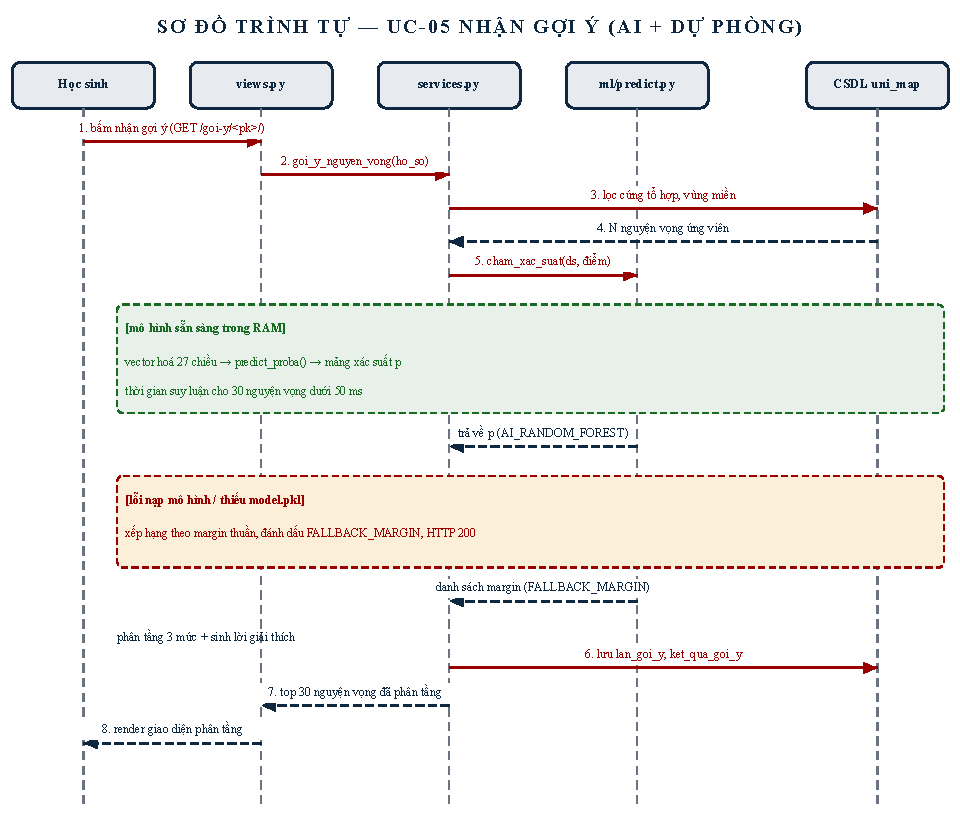
\includegraphics[width=\textwidth]{figs/svg/h-seq-goiy.pdf}
\caption{Sơ đồ trình tự UC-05 Nhận gợi ý (AI dự phòng xếp hạng theo margin khi lỗi mô hình).}
\label{fig:seq-goiy}
\end{figure}

\subsection{UC-09 + UC-10 Cập nhật dữ liệu và huấn luyện lại mô hình}

Luồng cập nhật dữ liệu năm mới và huấn luyện lại mô hình AI.

\begin{figure}[H]
\centering
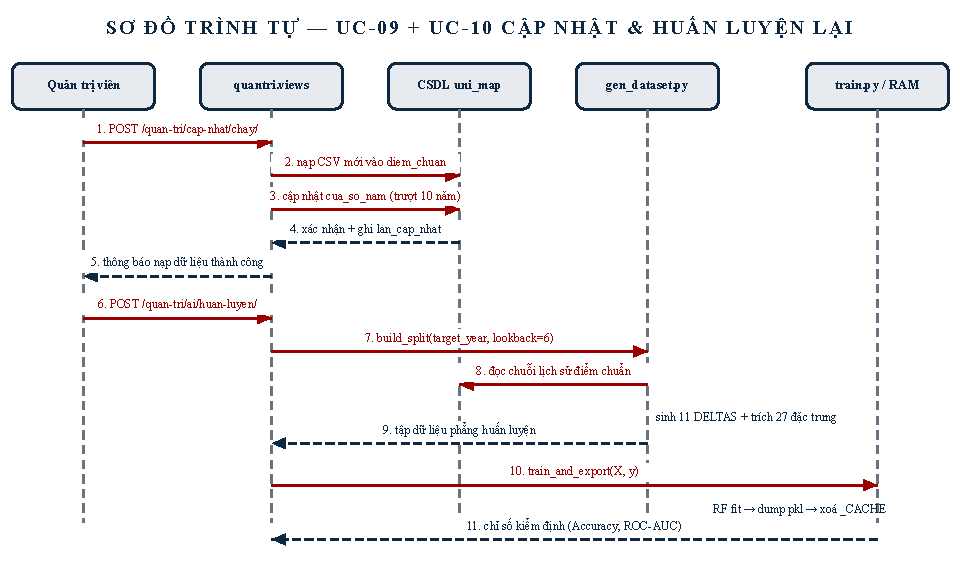
\includegraphics[width=\textwidth]{figs/svg/h-seq-capnhat.pdf}
\caption{Sơ đồ trình tự UC-09 + UC-10 Cập nhật dữ liệu năm mới và huấn luyện lại mô hình AI.}
\label{fig:seq-capnhat}
\end{figure}

Chi tiết định tuyến từ yêu cầu HTTP tới từng tầng xử lý được thể hiện ở Hình~\ref{fig:api}. Toàn bộ endpoint trong sơ đồ đều lấy nguyên văn từ bảy file \code{urls.py} của các ứng dụng Django (\code{university}, \code{api}, \code{accounts}, \code{admissions}, \code{recommendation}, \code{quantri}).

\begin{figure}[H]
\centering
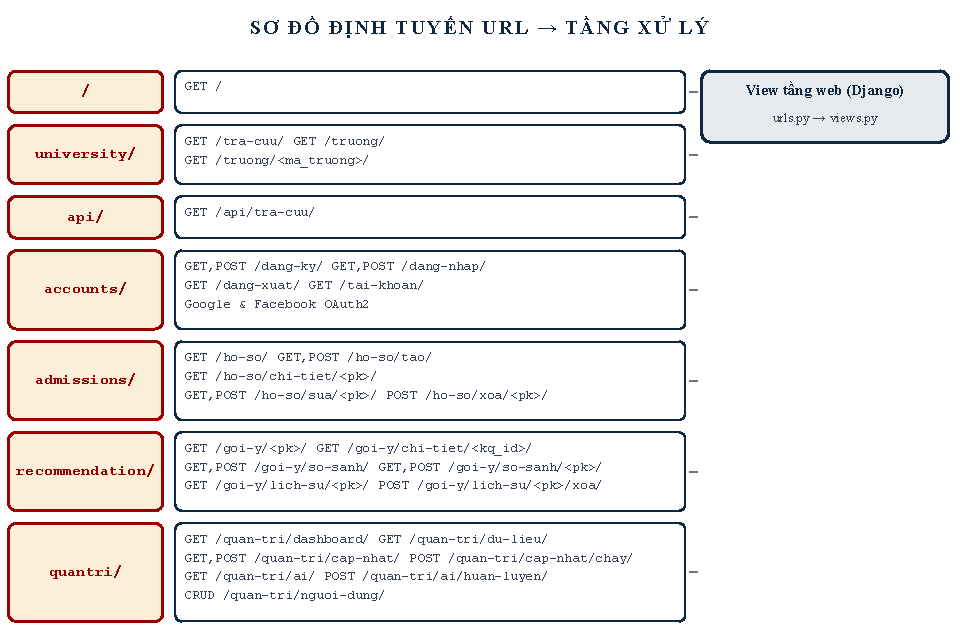
\includegraphics[width=\textwidth]{figs/svg/h-api.pdf}
\caption{Sơ đồ định tuyến API và URL của hệ thống Uni Connect.}
\label{fig:api}
\end{figure}

\section{Thiết kế dữ liệu}

\subsection{Nguồn và quy mô dữ liệu}

Dữ liệu điểm chuẩn được thu thập từ cổng tổng hợp \code{diemthi.tuyensinh247.com}. Quy trình thu thập tự động xử lý các tình huống thực tế phức tạp như lỗi font chữ tiếng Việt của nguồn, cơ chế công bố điểm nhỏ giọt kéo dài suốt mùa tuyển sinh và tự động chặn các năm chưa đủ dữ liệu tin cậy. Tổng quy mô dữ liệu thực tế sau khi chuẩn hóa được thống kê ở Bảng~\ref{tab:dulieu}.

\begin{table}[H]
\centering
\caption{Quy mô cơ sở dữ liệu điểm chuẩn thực tế của hệ thống Uni Connect.}
\label{tab:dulieu}
\begin{tabularx}{\textwidth}{>{\bfseries\color{daunavy}}l >{\color{daumaroon}\bfseries}r >{\raggedright\arraybackslash}X}
\toprule
\rowcolor{gray100}\bfseries\color{daunavy}Hạng mục dữ liệu & \bfseries\color{daumaroon}Số lượng & \bfseries\color{daunavy}Ghi chú \\
\midrule
Trường đại học         & 295        & Mã trường là khóa chính, phủ 3 miền Bắc -- Trung -- Nam \\
Ngành đào tạo          & 3.037      & Gom nhóm thành 15 nhóm ngành chuẩn \\
Tổ hợp xét tuyển       & 340        & Ví dụ: A00, B00, D01, C00 \\
Bản ghi điểm chuẩn     & 240.483    & Fact (trường, ngành, tổ hợp, phương thức, năm) \\
Chuỗi đặc trưng        & 100.363    & Dòng thống kê chuỗi 10 năm cho mỗi nguyện vọng \\
Cửa sổ dữ liệu         & 2016--2025 & 10 năm liên tục, hiển thị đầy đủ; AI dùng 6 năm gần nhất \\
\bottomrule
\end{tabularx}
\end{table}

\subsection{Lược đồ cơ sở dữ liệu}

\begin{figure}[H]
\centering
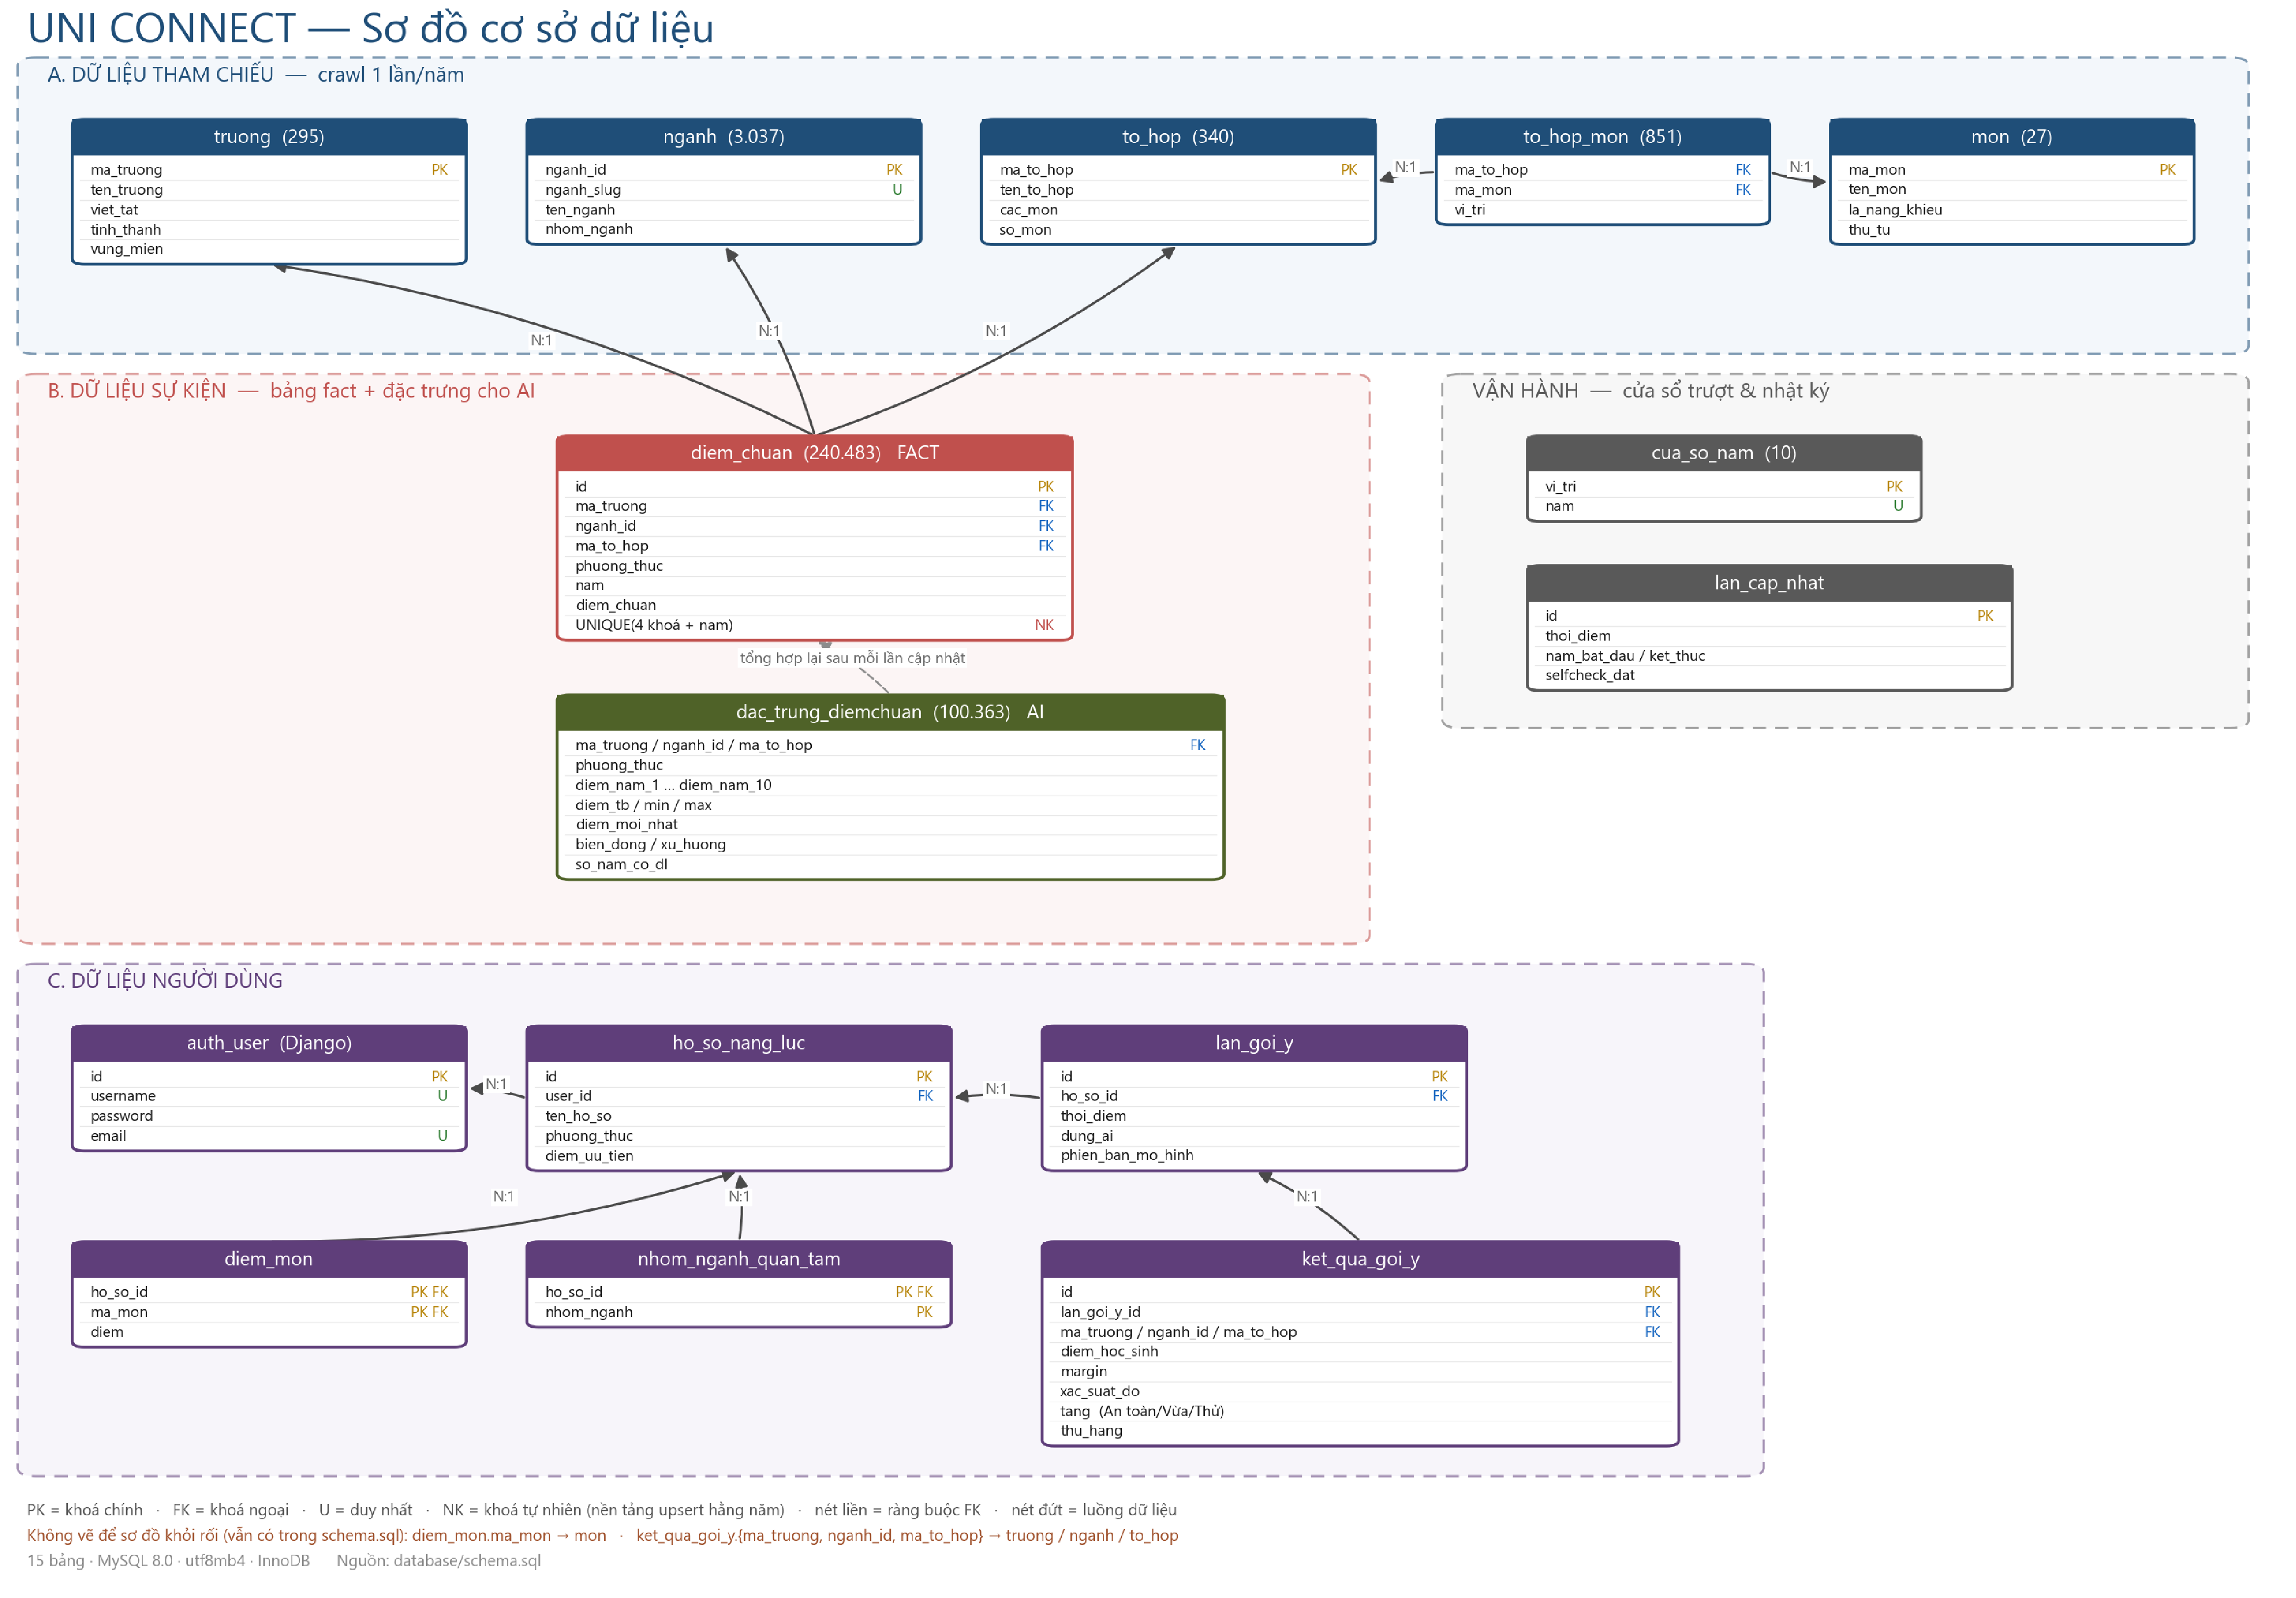
\includegraphics[width=\textwidth]{figs/svg/h-erd-source.pdf}
\caption{Lược đồ quan hệ ERD của cơ sở dữ liệu \code{uni_map}, lấy từ sơ đồ CSDL thực tế của hệ thống.}
\label{fig:erd}
\end{figure}

Cơ sở dữ liệu quan hệ \code{uni_map} bao gồm 15 bảng, quan hệ giữa chúng được
tóm tắt ở Hình~\ref{fig:erd}. Trong đó \code{db/schema.sql} là nguồn chân lý duy
nhất của lược đồ (các model Django đặt \code{managed = False} và không sinh
migration cho các bảng nghiệp vụ) --- cùng nguyên tắc tách lược đồ khỏi mã ứng
dụng được bàn trong~\cite{Fowler2002}.

Hình~\ref{fig:erd} chia 15 bảng thành bốn nhóm chức năng, và cách chia này phản
ánh trực tiếp vòng đời dữ liệu của hệ thống. Nhóm \en{tham chiếu} gồm
\code{truong}, \code{nganh}, \code{mon}, \code{to_hop} và \code{to_hop_mon} quản
lý danh mục và chỉ thay đổi khi có trường hoặc ngành mới. Nhóm \en{sự kiện} gồm
\code{diem_chuan} --- bảng fact trung tâm lưu điểm trúng tuyển của từng bộ
(trường, ngành, tổ hợp, phương thức, năm) --- và \code{dac_trung_diemchuan} lưu
10 cột điểm thô \code{diem_nam_1} đến \code{diem_nam_10} cùng các chỉ số thống
kê đã tính sẵn (\code{diem_tb}, \code{diem_min}, \code{diem_max},
\code{diem_moi_nhat}, \code{bien_dong}, \code{xu_huong}, \code{so_nam_co_dl}).
Nhóm \en{vận hành} gồm \code{cua_so_nam} và \code{lan_cap_nhat} phục vụ cơ chế
trượt cửa sổ và ghi vết mỗi lần nạp dữ liệu. Nhóm \en{người dùng} gồm
\code{auth\_user} của Django cùng bốn bảng hồ sơ và kết quả gợi ý
(\code{ho_so_nang_luc}, \code{diem_mon}, \code{nhom_nganh_quan_tam},
\code{lan_goi_y}, \code{ket_qua_goi_y}).

Điểm thiết kế nổi bật là bảng \code{cua_so_nam} ánh xạ vị trí cột ($1$--$10$) sang năm thực tế (2016--2025). Khi cập nhật dữ liệu năm 2026, quản trị viên chỉ cần thay đổi ánh xạ này qua giao diện mà hệ thống tự trượt cửa sổ hiển thị, không cần thực hiện lệnh \code{ALTER TABLE} hay sửa đổi mã nguồn (yêu cầu CN-05).

\section{Thiết kế mô hình và bộ đặc trưng}

\subsection{Chiến lược sinh nhãn huấn luyện}

Do không tồn tại dữ liệu đỗ/trượt thực tế của thí sinh trong quá khứ (giả định GĐ-3), đồ án áp dụng kỹ thuật sinh mẫu giả lập từ lịch sử: mỗi bản ghi điểm chuẩn $C$ của năm mục tiêu $t$ được xem là một ``sự thật tuyển sinh'' --- thí sinh giả lập có điểm thi $X$ xung quanh $C$ sẽ đỗ nếu $X \ge C$. Cụ thể, với mỗi nguyện vọng, 11 mức chênh lệch \code{DELTAS} $= \{-3{,}0; -2{,}0; -1{,}0; -0{,}5; -0{,}2; 0{,}0; +0{,}2; +0{,}5; +1{,}0; +2{,}0; +3{,}0\}$ được cộng vào điểm chuẩn gốc để tạo ra 11 mẫu huấn luyện có nhãn cân bằng.

Để ngăn chặn tuyệt đối hiện tượng rò rỉ dữ liệu \en{(data leakage)} --- hiện
tượng đã được phân loại và mô tả có hệ thống trong~\cite{Kaufman2012} --- đặc
trưng của mẫu năm mục tiêu $t$ chỉ được phép tính toán từ các năm quá khứ nhỏ
hơn $t$. Đồng thời, tập dữ liệu được chia cứng theo mốc thời gian: huấn luyện
trên các năm 2021--2024 và kiểm thử hoàn toàn độc lập trên năm 2025. Cách chia
này khác với kiểm định chéo $k$-fold thông thường: nếu trộn ngẫu nhiên các mẫu
của mọi năm rồi chia $k$ phần, mẫu của năm 2025 sẽ xuất hiện trong cả tập huấn
luyện lẫn tập kiểm thử và kết quả đo trở nên vô nghĩa.

\subsection{Bộ 27 đặc trưng và siêu tham số}

Vector đầu vào của mô hình gồm 27 chiều, thứ tự được cố định nghiêm ngặt trong file \code{constants.py} để đảm bảo tính nhất quán giữa giai đoạn huấn luyện và suy luận: 7 đặc trưng số (\code{diem_thi}, \code{margin}, \code{diem_moi_nhat}, \code{diem_tb}, \code{xu_huong}, \code{bien_dong}, \code{so_nam_co_dl}), 15 cột mã hóa \en{one-hot} nhóm ngành, 3 cột vùng miền và 2 cột phương thức xét tuyển. Bảng~\ref{tab:dactrung} liệt kê đầy đủ 27 đặc trưng theo bốn nhóm cùng vai trò của từng nhóm trong bài toán dự đoán.

\begin{table}[H]
\centering
\caption{Bộ 27 đặc trưng đầu vào của mô hình, chia thành bốn nhóm theo bản chất thông tin.}
\label{tab:dactrung}
\small
\begin{tabularx}{\textwidth}{@{}>{\raggedright\arraybackslash\strut}p{2.45cm}
  >{\centering\arraybackslash\strut}p{1.05cm}
  >{\raggedright\arraybackslash\strut}X
  >{\raggedright\arraybackslash\strut}p{3.15cm}@{}}
\toprule
\rowcolor{gray100}\bfseries\color{daunavy}Nhóm đặc trưng &
\bfseries\color{daumaroon}Số chiều &
\bfseries\color{daunavy}Thành phần (tên cột trong \code{constants.py}) &
\bfseries\color{daunavy}Vai trò trong dự đoán \\
\midrule
Đặc trưng số & 7 &
\code{diem_thi}, \code{margin}, \code{diem_moi_nhat}, \code{diem_tb},
\code{xu_huong}, \code{bien_dong}, \code{so_nam_co_dl} &
Mô tả trực tiếp năng lực thí sinh và diễn biến lịch sử của ngành \\
\addlinespace[2pt]
Nhóm ngành & 15 &
Mã hóa \en{one-hot} cho 15 nhóm ngành chuẩn, tiền tố \code{nn_}:
Báo chí -- Truyền thông; Công nghệ thông tin; Du lịch -- Khách sạn -- Nhà hàng;
Khác; Khoa học XH \& Nhân văn; Kiến trúc -- Xây dựng; Kinh tế -- Kinh doanh -- Tài chính;
Kỹ thuật -- Công nghệ; Luật; Nghệ thuật -- Thiết kế -- TDTT; Ngôn ngữ -- Quốc tế học;
Nông -- Lâm -- Ngư -- Thú y; Quân đội -- Công an; Sư phạm -- Giáo dục; Y -- Dược -- Sức khỏe &
Phản ánh mức cạnh tranh đặc thù của từng lĩnh vực đào tạo \\
\addlinespace[2pt]
Vùng miền & 3 &
\code{vm_Miền Bắc}, \code{vm_Miền Trung}, \code{vm_Miền Nam} &
Hiệu chỉnh khác biệt mặt bằng điểm theo khu vực địa lý \\
\addlinespace[2pt]
Phương thức & 2 &
\code{pt_Điểm thi THPT}, \code{pt_Điểm học bạ} &
Phân biệt khác biệt về thang điểm và phân bố giữa hai phương thức \\
\midrule
\rowcolor{gray100}\bfseries Tổng cộng & \bfseries\color{daumaroon}27 &
\bfseries 7 số + 15 nhóm ngành + 3 vùng miền + 2 phương thức &
\bfseries Thứ tự cố định, khớp tuyệt đối giữa huấn luyện và suy luận \\
\bottomrule
\end{tabularx}
\end{table}

Bảng~\ref{tab:dactrung} cho thấy bốn nhóm đặc trưng không ngang hàng về số chiều nhưng bổ sung cho nhau theo ba lớp thông tin. Lớp thứ nhất là năng lực cá nhân, gồm \code{diem_thi} và \code{margin} --- hai biến quyết định phần lớn kết quả dự đoán. Lớp thứ hai là bối cảnh lịch sử của ngành, gồm bốn chỉ số thống kê chuỗi thời gian còn lại. Lớp thứ ba là bối cảnh phân loại, gồm 20 cột \en{one-hot} cho nhóm ngành, vùng miền và phương thức xét tuyển. Việc tách 15 nhóm ngành thành 15 cột nhị phân thay vì một cột số nguyên là lựa chọn có chủ đích: cây quyết định chỉ so sánh được ngưỡng số, nên nếu mã hóa nhóm ngành thành các số 1--15 thì mô hình sẽ ngầm hiểu nhóm 15 ``lớn hơn'' nhóm 1 --- một quan hệ thứ tự không có thật trong dữ liệu. Mã hóa \en{one-hot} loại bỏ giả định sai này, đổi lại làm số chiều tăng từ 10 lên 27. Chi phí đó được chấp nhận vì với 27 chiều và hơn 900 nghìn mẫu huấn luyện, Random Forest vẫn hội tụ ổn định và thời gian suy luận cho 30 nguyện vọng vẫn dưới 50 mili-giây.

Trong đó, \code{margin} (điểm thí sinh trừ điểm chuẩn mới nhất) là đặc trưng trung tâm phản ánh trực tiếp khoảng cách năng lực; \code{xu_huong} là độ dốc hồi quy tuyến tính của chuỗi điểm phản ánh mức độ cạnh tranh ngày càng tăng; \code{bien_dong} là hiệu số điểm lớn nhất trừ nhỏ nhất phản ánh mức độ rủi ro khó đoán.

Mô hình chính \code{RandomForestClassifier} được chốt siêu tham số: \code{n_estimators=100} cây, \code{min_samples_leaf=5}, \code{max_depth=14} và \code{random_state=42}. Cấu hình này là kết quả cân bằng giữa độ chính xác và ràng buộc kích thước file mô hình dưới 100~MB để có thể triển khai trên máy chủ phổ thông. Mô hình đối chứng \code{DecisionTreeClassifier} dùng chung \code{min_samples_leaf=5} để so sánh công bằng. Mọi đặc trưng số đều được chuẩn hóa bằng \code{StandardScaler} trước khi đưa vào huấn luyện.

\section{Thiết kế luồng giao diện}

Sơ đồ luồng giao diện ở Hình~\ref{fig:ifd} mô tả đường đi của người dùng qua bốn nhóm màn hình chính: khu vực khách tra cứu công khai, khu vực tài khoản, khu vực hồ sơ và gợi ý dành cho học sinh đã đăng nhập, và khu vực quản trị. Đường nét liền biểu diễn luồng điều hướng chính, đường nét đứt biểu diễn luồng phụ hoặc luồng quay về. Mỗi màn hình đều ghi kèm đường dẫn URL tương ứng để đối chiếu trực tiếp với mã nguồn.

\begin{figure}[H]
\centering
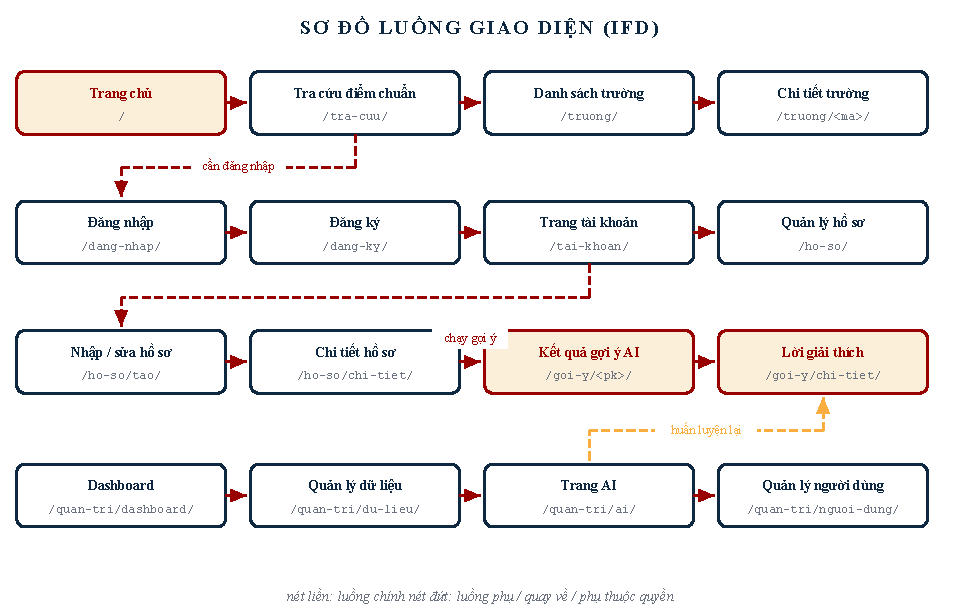
\includegraphics[width=\textwidth]{figs/svg/h-ifd.pdf}
\caption{Sơ đồ luồng giao diện (IFD) của hệ thống Uni Connect.}
\label{fig:ifd}
\end{figure}

Luồng nghiệp vụ trung tâm đi từ màn hình chi tiết hồ sơ sang trang kết quả gợi ý, tại đây hệ thống gọi mô hình để sinh xác suất trúng tuyển và phân tầng kết quả. Từ trang kết quả, học sinh có thể mở trang lời giải thích chi tiết cho từng nguyện vọng, chuyển sang màn hình so sánh nhiều nguyện vọng cạnh nhau, hoặc truy cập lại lịch sử các lần gợi ý trước đó.
